
\section{Requirements}

In order to satisfy goals in section {[}Section Goals{]} under domain
assumptions in Section {[}Section domain Assumption{]} we've derived
requirements for our system.
\begin{itemize}
\item {[}G1.1{]} Only USER should be able to reserve a car:
\begin{itemize}
\item {[}R1{]} The system can modify car's status (available, occupied,
in use).
\item {[}R2{]} The system shall be able to know car's status.
\item {[}R2{]} The system shall reserve a car only if the car is available. 
\item {[}R3{]} The system shall be able to associate a car to the USER who
has reserved it. 
\item {[}R\_{]} The system shall provide the login functionality.
\item {[}R\_{]} The system shall provide sign up functionality.
\end{itemize}
\item {[}G1.2{]} USER should be able to unlock reserved car when they are
close to it.
\begin{itemize}
\item {[}R4{]} The system shall know cars' location according to cars' GPS.
\item {[}R5{]} The system shall know user's location according to his GPS.
\item {[}R6{]} The system shall provide a functionality to unlock the car. 
\item {[}D1{]}
\item {[}D2{]}
\item {[}D3{]}
\end{itemize}
\item {[}G1.3{]} USER should be aware of how much they are going to pay
during the ride.
\begin{itemize}
\item {[}R7{]} The system shall be able to calculate ride's cost based on
duration.
\item {[}R8{]} The system shall be able to communicate to the car ride's
cost.
\item {[}D4{]}
\end{itemize}
\item {[}G2{]} The reservation of two (or more) cars at a time must be forbidden.
\begin{itemize}
\item {[}R7{]} The system shall reserve a car only if the user hasn't already
reserved another car.
\item {[}R3{]}
\end{itemize}
\item {[}G3.1{]} USER or GUEST should be able to search car near his position.
\begin{itemize}
\item {[}R4{]}
\item {[}R5{]}
\item {[}R9{]} The system shall provide the closest cars to user's position.
\end{itemize}
\item {[}G3.2{]} USER or GUEST should be able to search car near a selected
position.
\begin{itemize}
\item {[}R4{]}
\item {[}R5{]}
\item {[}R10{]} The system shall provide the closest cars to position provided
by the USER.
\end{itemize}
\item {[}G4.1{]} A discount of 10\% should be applied to rides with at least
two passengers. 
\begin{itemize}
\item {[}R11{]} The system shall bel able to detect if there are at least
two passengers in the car.
\item {[}D5{]}
\item {[}R12{]} The system shall be able to apply a discount on the ride.
\end{itemize}
\item {[}G4.2{]} If a car is left with no more than 50\% battery empty,
a discount of 20\% should be applied to the last ride.
\begin{itemize}
\item {[}R13{]} The system shall be able to know the battery level of the
car.
\item {[}R12{]}
\item {[}D7{]}
\end{itemize}
\item {[}G4.3{]} If a car is left at more than 3 km from the nearest charging
area, the system should charge 30\% more on the last ride.
\begin{itemize}
\item {[}R4{]}
\item {[}R13{]}
\item {[}R14{]} The system shall be able to apply a charge on the ride.
\item {[}R15{]} The system shall be able to calculate distance between car's
position and the nearest charging area.
\end{itemize}
\item {[}G4.4{]} If a car is left with more than 80\% battery empty, the
system should charges 30\% more on the last ride. 
\begin{itemize}
\item {[}R13{]}
\item {[}R14{]}
\end{itemize}
\item {[}G4.5{]} If a car is left in a charging area and the user plugs
the car into the power grid, a discount of 30\% should be applied
to the last ride.
\begin{itemize}
\item {[}R15{]} The system shall be able to detect if the user has plugged
the car into the power grid.
\item {[}R12{]}
\item {[}R4{]}
\item {[}D6{]}
\end{itemize}
\item {[}G4.6{]} If a car is not picked up within one hour from the reservation,
the user pays a fee of 1 EUR.
\begin{itemize}
\item {[}R16{]} The system shall be able to monitor car's reservations.
\item {[}R17{]} The system shall be able to know if a user has picked up
a car. 
\item {[}R2{]}
\end{itemize}
\item {[}G4.7{]} If a payment fails for a insufficient money availability
of the USER, the USER should be suspended from the service until the
payment is done.
\begin{itemize}
\item {[}R18{]} The system shall take care of the result of the payment.
\item {[}R19{]} The system shall suspend USER that can't afford the payment.
\item {[}R20{]} The system shall unsuspend a USER when his old undone payment
is done.
\end{itemize}
\item {[}G5{]} USER have to pay an amount of money based on the ride's duration.
\begin{itemize}
\item {[}R7{]} 
\item {[}R21{]} The system shall charge an extenernal payment service with
doing the payment.
\item {[}R9{]}
\item {[}D4{]} 
\end{itemize}
\item {[}G6.1{]} Only OPERATOR must be able to do car mantainance, knowing
their position and status.
\begin{itemize}
\item {[}R22{]} The system shall offer a backend panel to Operator
\item {[}R23{]} The system shall notify the operator when a car in his competence
area needs some kind of maintenance.
\item {[}D7{]} 
\item {[}D8{]}
\item {[}D9{]}
\item {[}D10{]}
\item {[}R1{]}
\item {[}R2{]}
\end{itemize}
\item {[}G6.2{]} USER must be able to communicate to the system cars damages
and malfunctions. 
\begin{itemize}
\item {[}R24{]} The system shall offer a functionality that let USERs to
comunicate malfunctions and damages.
\end{itemize}
\item {[}G7.1{]} Only ADMIN must be able to manage safe areas.
\begin{itemize}
\item {[}R25{]} The system shall offer the functionality of add or remove
safe areas.
\item {[}R26{]} The system shall offer log in functionality for admin.
\item {[}D11{]}
\end{itemize}
\item {[}G7.2{]} Only ADMIN must be able to manage OPERATORs.
\begin{itemize}
\item {[}R26{]}
\item {[}R27{]} The system shall offer the functionality of add or remove
safe areas
\item {[}D11{]}
\end{itemize}
\end{itemize}

\subsection{Functional Requirements}

After having defined main features of our system we can identify some
functional requirements grouped under each defined actor:
\begin{itemize}
\item GUEST, he can:
\begin{itemize}
\item Sign up.
\item Search for a car near his location.
\item Search for a car near a selected location.
\end{itemize}
\item USER, he can:
\begin{itemize}
\item Log in.
\item Reserve cars.
\item Use a reserved car (unlocking it).
\item View his profile (also his discounts).
\item Modify his profile.
\item View his recent reservations.
\item Search cars near to his location.
\item Search cars near a selected location.
\item Communicate malfunction or damages to the system.
\end{itemize}
\item OPERATOR, he can:
\begin{itemize}
\item Log in.
\item View car's status (battery and location).
\item Receive notification when a car need to be charged.
\item Set a car as available or under maintainance.
\end{itemize}
\item ADMIN, he can:
\begin{itemize}
\item Log in.
\item Add or delete safe areas.
\item Manage car status.
\item Consult car position.
\item Add or delete OPERATORs account.
\item Manage other ADMINs.
\end{itemize}
\end{itemize}

\subsection{Non-functional Requirements}

\subsubsection{User Interface}
\begin{flushleft}
In order to make PowerEnJoy available for many people as possible,
a Cross-Platform application has to be developed, with a Framework
like Xamarin. In this way, a single application could be developed
and then deployed for Windows Phone, Android and iOS. A Web Application
has also to be developed in order to allow people to use our system
in many way as possible.\\
The User Interface needs to be as user friendly as possible: that's
to say that a user who uses Power EnJoy for the first time should
be able to learn in a few seconds how to make use of it. \\
Here are presented a few screen of the app to provide an example.
\par\end{flushleft}

\begin{center}
\begin{figure}[H]
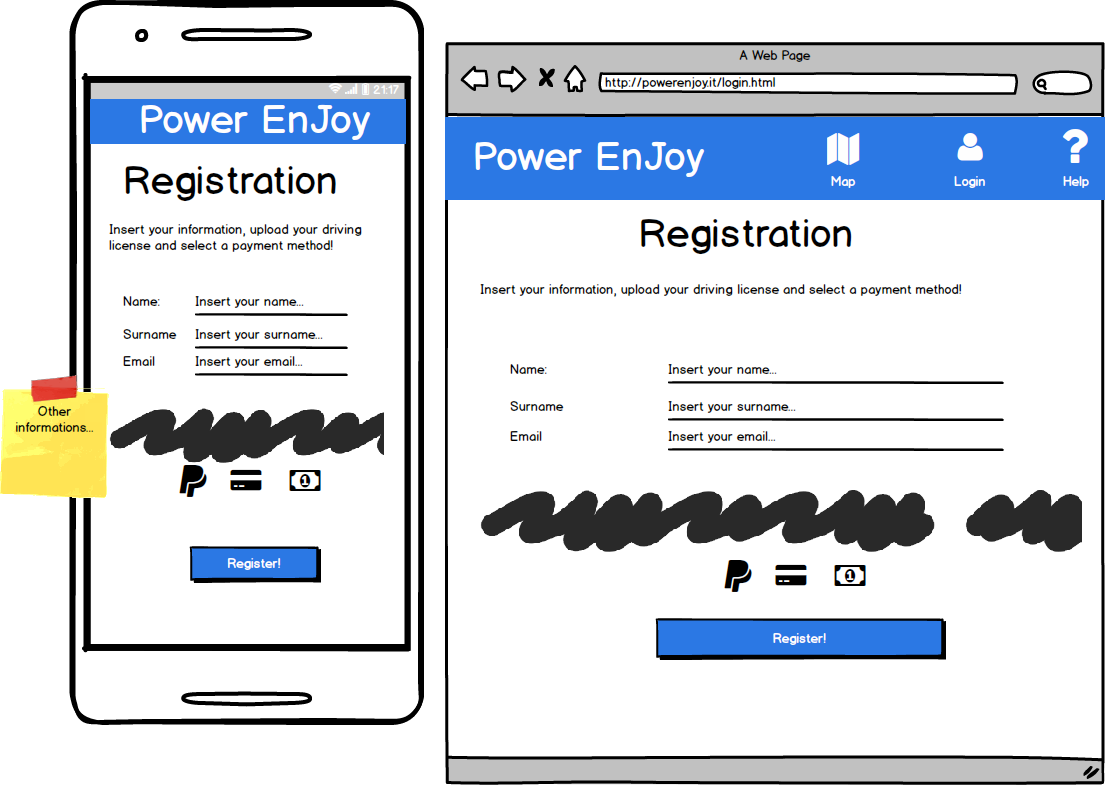
\includegraphics[scale=0.3]{Mockup/Register}

\caption{Registration}

\end{figure}
\\
\\
\begin{figure}[H]
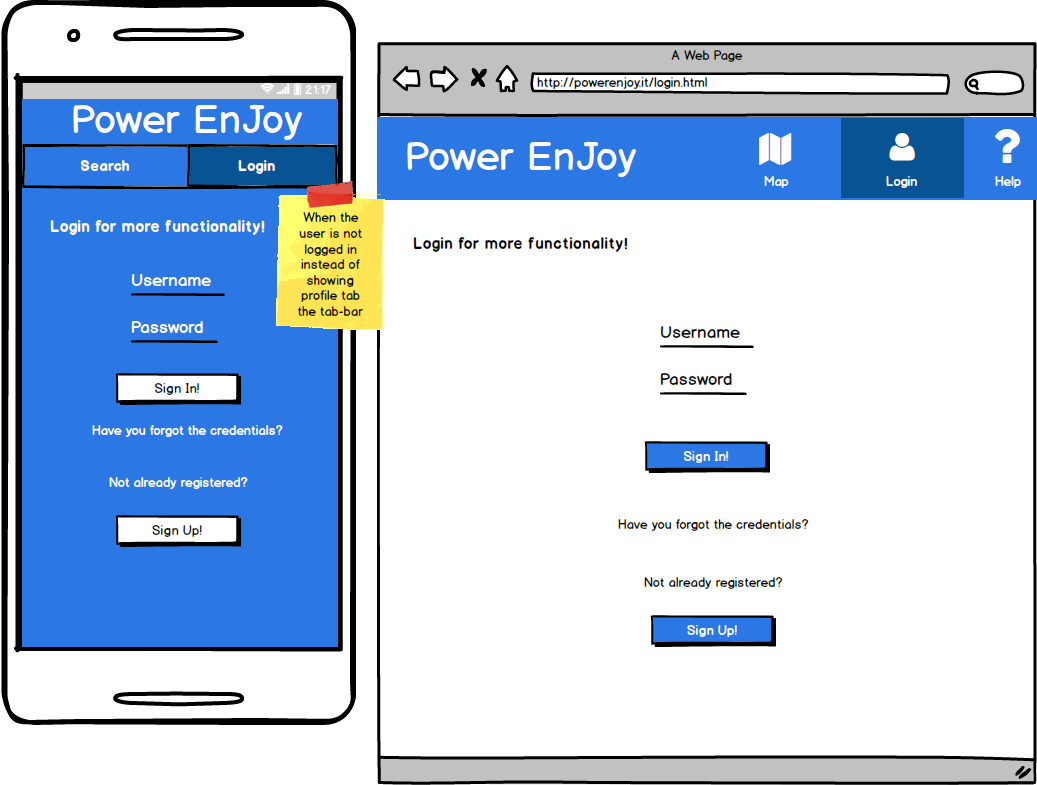
\includegraphics[scale=0.3]{Mockup/Login}

\caption{Login}

\end{figure}
\\
\\
\par\end{center}

\begin{center}
\begin{figure}[H]
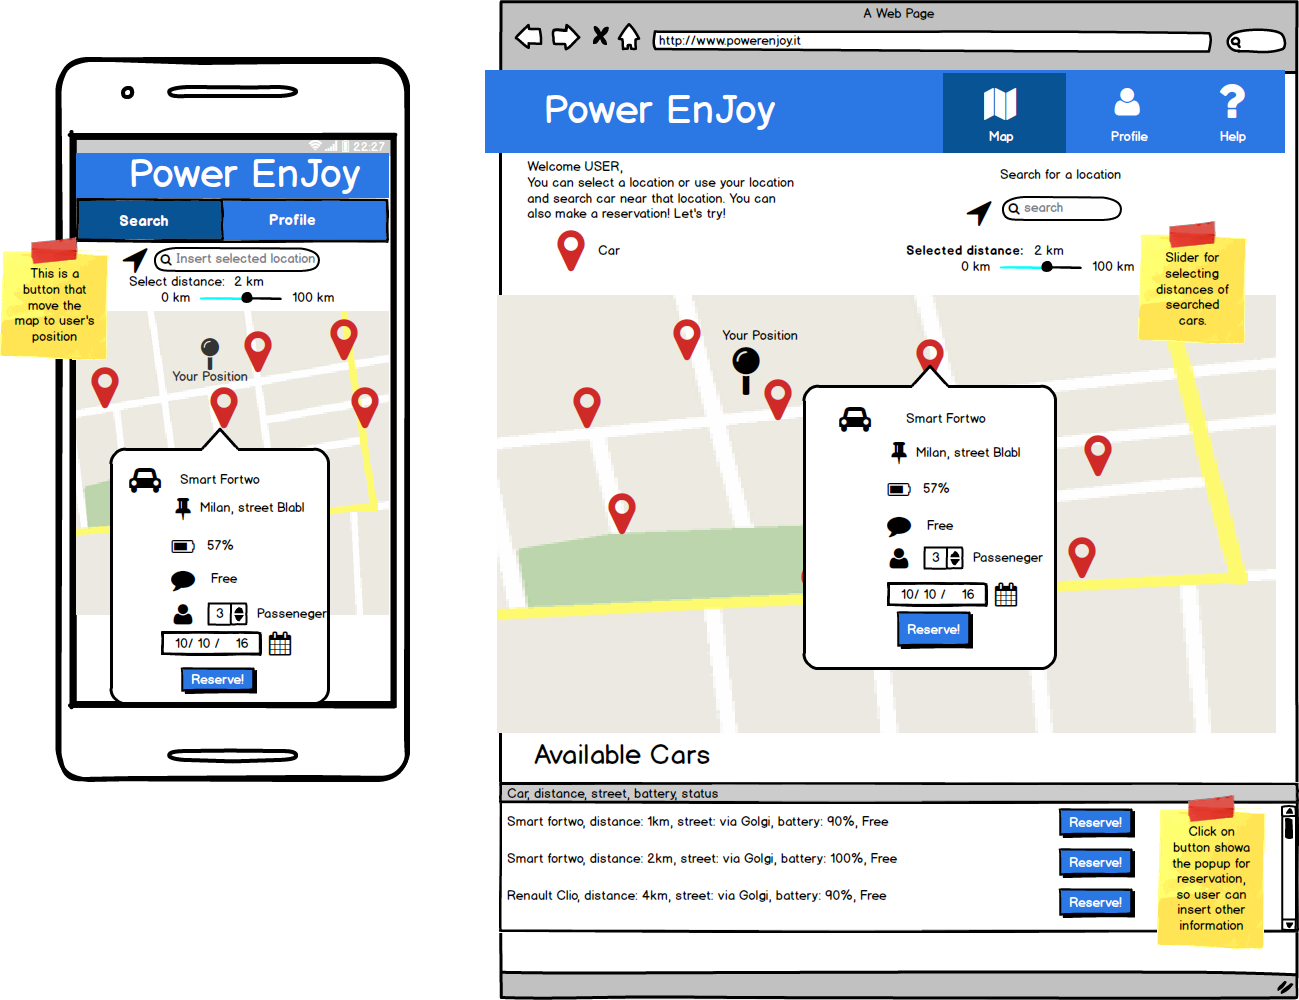
\includegraphics[scale=0.15]{Mockup/Map}

\caption{Map UI}
\end{figure}
\\
\\
\begin{figure}[H]

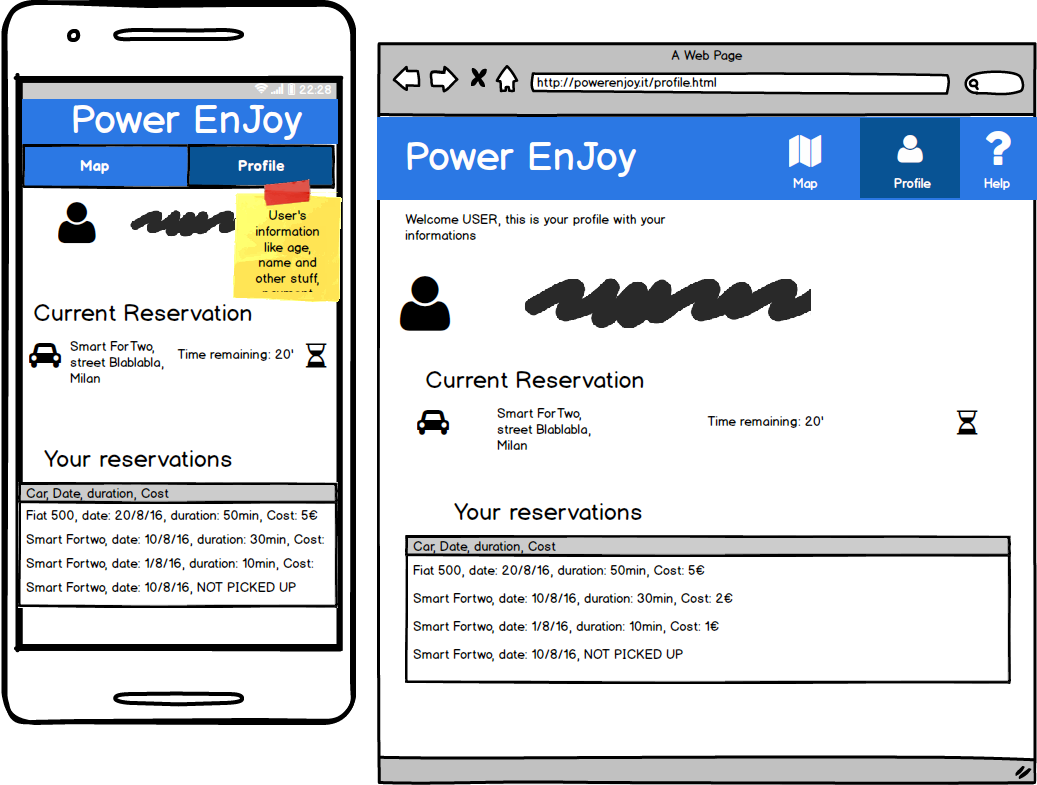
\includegraphics[scale=0.3]{Mockup/Profile}

\caption{User Profile}
\end{figure}
\\
\\
\begin{figure}[H]

\includegraphics[scale=0.3]{\string"Mockup/Admin Panel\string".png}

\caption{Admin Panel}

\end{figure}
\\
\\
\begin{figure}[H]

\includegraphics[scale=0.3]{\string"Mockup/Operator Panel\string".png}

\caption{Operator Panel}

\end{figure}
\par\end{center}

\subsubsection{Security}

The system has to satisfy an high level of security regarding the
communication protocol with the cars.\\
The communication with the cars needs to be encrypted in order to
avoid unauthorized unlocks and use. Futhermore the system should have
the way to stop cars when used in an unauthorized way.\\
Regarding the security of payment, the system does't care about it
because it relies on external payment system.\\
Another critical security point is the managing of user's information:
all user informations need to be encrypted before being sent. 

\subsubsection{Availability}

The application needs to be online 24h/day and 7day/week in order
to satisfy all users. This is a constraints because an hour of unavailablity
could induce users to use another car sharing service. To achieve
an high level of availability could be necessary to use a dedicated
server and all the system could be hosted in a cloud platform like
OVH. The system should be able to support a high number of users connected
at the same time and could be necessary to scale resources depending
on this. 

\subsubsection{Portability}

The client-part of the system (application) could be used on any mobile
OS in order to make it available for as many people as possible. It
is expected a Web Application to increase the possible number of users.\\
The server-part of the system could be used on any OS which supports
JVM and DBMS.

\subsubsection{Maintainability}

The system code will be documented in order to make easier future
improvements or changes by other developers. It needs to be clear
how the system works, how the system communicate with cars, and how
the system has been developed.

\subsubsection{Documentation}

These documents will be released in order to well-organize the work
in the way to obtain the best quality-cost ratio as possible:
\begin{itemize}
\item $\boldsymbol{RASD}$: Requirements Analysis and Specification Document,
to well-understand the given problem and to analyze system's boundaries
and goal. RASD is also important to understan system's requirements
and specifications in order to reach the goals.
\item $\mathbf{\boldsymbol{DD}}:$Design Document, to define the structure
of the the system, his tiers, and the interaction between them.
\item $\boldsymbol{ITPD}$: Integration Test Plan Document, to describe
the planning to accomplish the integration test. This document is
supposed to be written before the integration test really happens.
Moreover this document needs to explain to the developer team what
to test, in which sequence, which tools are needed for testing and
wich need to be developed.
\item $\boldsymbol{PP}$: Project Plan, aims at defining a planning for
the project. It regards in particular the estimation of effort and
cost, the scheduling for project's task and the allocation of resources
to tasks. 
\end{itemize}

